\section{Higgs zero mode IV: survival along the turn}\label{rep:h-survival}

Along the turn the couplings run and the conformal time is finite, so the zero mode decays with a time-dependent hazard.
We show that the hazard gives the survival probability of the resonant component of a time-symmetric real state, exactly in the adiabatic limit and to $0.2\%$ in a real-time evolution of the final model, that the minimal-variance rule of assumption (A8) fixes the weight of that component to $w_0=0.980$--$0.995$, and that the criterion barely depends on this weight. %
For a Higgs curvature coupling $\xiH<1/6$ the late turn adds an inverted oscillator, which we follow with an exact lens transformation and a quantum--classical switch; this machinery fixes the threshold $\xic$ of Sec.~\ref{rep:h-universality}.
Finally we show that the joint survival of both branches of the turning point has no probability in the decoherent-histories sense, so we quote single-branch probabilities throughout.
These are the measure statements of assumption (A4) of Sec.~\ref{rep:setup}.

\subsection{The turn as seen by the zero mode}
\label{sec:rb-turn}

The turning solution of Sec.~\ref{rep:turning} is $a^2=\cosh2\tau$ with $\tau\equiv ht$, so the edge of the torus grows as $L(\tau)=\Lb(\cosh2\tau)^{1/2}$.
Two consequences follow for the zero-mode problem, which lives in units of $1/L$.
First, the zero mode sees the Standard Model couplings at
\begin{equation}
\mu(\tau)=\frac{\mub}{(\cosh2\tau)^{1/2}},
\label{eq:rb-mutau}
\end{equation}
which we call the nodes of the hazard.
Second, its natural clock is the conformal time measured in units of $\Lb$.
With $d\eta=dt/(a\Lb)$,
\begin{equation}
d\eta=\frac{d\tau}{h\Lb(\cosh2\tau)^{1/2}},\qquad
\eta_\infty=\frac{1}{h\Lb}\int_0^\infty\frac{d\tau}{(\cosh2\tau)^{1/2}}=\frac{\Gamma(\frac14)^2}{4\sqrt{2\pi}\,h\Lb}=\frac{1.31103}{h\Lb}, %
\label{eq:rb-etainf}
\end{equation}
where we used $\int_0^\infty\cosh^{-\nu}x\,dx=2^{\nu-2}\Gamma(\nu/2)^2/\Gamma(\nu)$ at $\nu=\frac12$.
With $h\Lb=0.00437243$ the conformal duration of one branch is $\eta_\infty=299.84$, and the nodes $\tau\le5$ cover all but $\sqrt2\,e^{-5}/1.31103=0.7\%$ of it. %
This value of $h\Lb$ differs by $1\%$ from the instantaneous-reheating normalization of Sec.~\ref{rep:turning}, which would shift $m_c$ by at most $0.002\GeV$. %
The turning solution also has constant curvature: from $\dot a/a=h\tanh2\tau$ and $\dot a^2+a\ddot a=2h^2\cosh2\tau$,
\begin{equation}
R=6\Bigl(\frac{\ddot a}{a}+\frac{\dot a^2}{a^2}\Bigr)=12h^2,\qquad \frac{a''}{a}=2h^2a^2\Lb^2=2(hL)^2,
\label{eq:rb-R}
\end{equation}
where a prime denotes $d/d\eta$; both relations are used for the curvature coupling in Sec.~\ref{sec:rb-late}.

\subsection{Hazard and single-branch survival probability}
\label{sec:rb-hazard}

At each of eleven nodes $\tau=0,0.5,\ldots,5$ we recompute the gauge profiles, the matching $\Delta V_{\rm MC}$, and the cross terms with the Standard Model couplings at $\mu(\tau)$, and we solve directly for the two-dimensional resonance (Sec.~\ref{sec:rb-nodes}).
The width $\Gamma(m_t,\tau)$ is a rate in conformal time, so the hazard and the single-branch survival probability are
\begin{equation}
I(m_t)=\int_0^5\frac{\Gamma(m_t,\tau)\,d\tau}{h\Lb(\cosh2\tau)^{1/2}},\qquad \Pone=e^{-I}.
\label{eq:rb-hazard}
\end{equation}
We interpolate $\ln\Gamma$ between the eleven nodes with a cubic spline, integrate with Simpson's rule on $20\,001$ points, and find $m_c$ as the root of a cubic spline of $\ln I$ in $m_t$ on the grid $172.0$--$173.8\GeV$. %
Twenty-nine nodes instead of eleven change $m_c$ by $7\times10^{-5}\GeV$. %
The hazard-equivalent threshold is the Standard Model quartic at $\mub$ evaluated at the critical mass, $\lamc(\mub)\equiv\lambda_{\rm SM}(\mub;m_c)=-0.0091$, $-0.0121$, and $-0.0152$ for $\Pone=0.9$, $0.5$, and $0.1$. %

If instead the width at $\tau=0$ were held for the whole branch, the static condition $\Gamma=-\ln P/\eta_\infty$, that is $\Gamma_c=3.514\times10^{-4}$ and $2.312\times10^{-3}$ for $P=0.9$ and $0.5$, would give the static thresholds $-0.00880$, $-0.01174$, and $-0.01472$ in the earlier model, which we quote only for comparison. %
Because $|\lambda(\mu)|$ and hence $\Gamma$ decrease along the turn, the static thresholds lie $0.0003$ to $0.0004$ above the hazard-equivalent ones of the same model. %
For the same reason the integrand of Eq.~(\ref{eq:rb-hazard}) is largest early in the turn [Fig.~\ref{fig:rb-hazard}(a)].
At $\alpha_s=0.1180$ we find $\Pone=0.9976$, $0.9850$, $0.9424$, $0.8426$, $0.6721$, $0.4549$, $0.2508$, $0.1093$, $0.0372$, and $0.0099$ for $m_t=172.0$ to $173.8\GeV$ in steps of $0.2\GeV$. %
Near the critical masses $d\ln I/dm_t=5.27$, $3.22$, and $2.12\GeV^{-1}$ at $\Pone=0.9$, $0.5$, and $0.1$, the slopes that convert width ratios into shifts of $m_c$ throughout Secs.~\ref{rep:h-reduced}--\ref{rep:h-budget}. %

\subsection{Real initial states and the survival measure}
\label{sec:rb-measure}

The width is a property of the resonance; the survival probability of a given state also depends on how much of it is resonant.
At $\tau=0$ the state of the zero mode is real and time-reflection invariant, $\psi(-\eta)=\psi(\eta)^*$.
We decompose it with the c-product $(\varphi,\psi)=\int\varphi\,\psi$ (no complex conjugation), under which the resonance $\varphi_{\rm res}$ is normalizable and orthogonal to the other eigenfunctions of the complex-symmetric Hamiltonian with an absorbing potential:
\begin{equation}
\psi_0=(\varphi_{\rm res},\psi_0)\,\varphi_{\rm res}+\psi_\perp,\qquad w_0\equiv|(\varphi_{\rm res},\psi_0)|^2 .
\label{eq:rb-decomp}
\end{equation}
The resonant part follows the instantaneous resonance adiabatically and loses norm at the hazard rate, while the non-resonant part $\psi_\perp$ lies above the barrier and leaves the well within $\Delta\eta\lesssim40$, about $\Delta\tau\lesssim0.2$. %
The in-well probability at the end of the branch is therefore
\begin{equation}
P_\infty=w_0\,P_{\rm haz,\infty}\,(1+\delta),\qquad P_{\rm haz}=\exp\Bigl(-\int\Gamma\,d\eta\Bigr),
\label{eq:rb-w0}
\end{equation}
where $\delta$ comes only from the definition of the in-well probability (cutting at the barrier top).

We verified Eq.~(\ref{eq:rb-w0}) by evolving real states with the time-dependent Schr\"odinger equation in the conformal frame.
The spatial discretization is a five-point fourth-order Laplacian with $dr=0.01$ up to $r=16$ and odd continuation at the origin, which gives the regular behavior $r^{s_0}$; time stepping is Crank--Nicolson with $d\eta=0.025$; beyond $r_c=10$, about twice the exit point, the potential is smoothly flattened and a quadratic absorbing potential removes the outgoing flux. %
The resonance is continued from node to node as an eigenvalue of the complex-symmetric Hamiltonian with the absorbing potential; its width agrees with the Siegert width to $0.2\%$ and its energy to $1.5\times10^{-6}$ at all nodes. %
In a one-dimensional model without cross terms, with the earlier mapping, the resonant projection decays at the hazard rate to $1.3\times10^{-4}$ for $\tau\le5$, and $|\delta|\le0.3\%$. %
Gamow-like states, the real part of the c-normalized resonance cut at the outer turning point or the ground state with a Dirichlet wall at $1.0$ or $1.2$ times the exit radius, have $w_0=0.9997$--$1.0019$ and $P_\infty/P_{\rm haz,\infty}-1\in[-0.34\%,+0.01\%]$. %
For every other real state we tried, the remainder decays at the hazard rate after the non-resonant part has left, so that $P_\infty=w_0P_{\rm haz,\infty}$.
An independent reimplementation reproduces $P_\infty=w_0P_{\rm haz,\infty}$ with projection deviations below $10^{-3}$; for the walled ground state at $1.2$ times the exit radius it finds $w_0=1.0019$ and $P_{\rm haz,\infty}=0.47706$ against $0.4770$ (Sec.~\ref{rep:v-blind}). %
In the final two-dimensional model the absorbing-potential pole at $\tau=0$ agrees with the Siegert root to $0.08\%$ in $\Gamma$, the Gamow-like state has $w_0=1.0000$--$1.0013$, and with $\xiH=1/6$ the real-time survival probability equals the hazard $\Pone$ to $0.22\%$. %
The hazard is therefore the survival measure conditional on the zero mode being in the metastable sector, and $w_0$ is a separate preparation factor.
We use only Lorentzian widths: a Euclidean preparation is ill defined for a negative quartic, and $w_0$ parametrizes the preparation instead.

\subsection{Preparation weight}
\label{sec:rb-w0}

For $P=w_0\Pone$ the critical masses depend on $w_0$ as in Table~\ref{tab:rb-w0}; for $w_0<0.9$ the level $P=0.9$ is never reached. %
The criterion barely depends on the preparation: even $w_0=0.9$ or $0.8$ would lower the critical mass for probability $1/2$ by only $0.050$ or $0.114\GeV$. %

\begin{table}[t]
\centering
\caption{Shift of the critical top mass (GeV) for a survival probability $P=w_0\Pone$, relative to $w_0=1$, at $\alpha_s(M_Z)=0.1180$, computed with the cross terms before their final one-loop corrections; for the minimal-variance weights the final model gives the same shifts to $0.001\GeV$.} %
\label{tab:rb-w0}
\begin{tabular}{cccc}
\toprule
$w_0$ & $P=0.9$ & $P=0.5$ & $P=0.1$ \\
\midrule
$0.99$ & $-0.019$ & $-0.005$ & $-0.002$ \\ %
$0.95$ & $-0.118$ & $-0.024$ & $-0.011$ \\ %
$0.9$ & --- & $-0.050$ & $-0.022$ \\ %
$0.8$ & --- & $-0.114$ & $-0.047$ \\ %
$0.55$ & --- & $-0.475$ & $-0.134$ \\ %
\bottomrule
\end{tabular}
\end{table}

To fix $w_0$ we apply to the Higgs zero mode the rule that selects the shape state at the turning point (assumption (A8) and Sec.~\ref{rep:quantum-shape}): among real, time-symmetric central Gaussians, take the one with the smallest instantaneous energy variance.
We use the two-dimensional model at $\tau=0$,
\begin{equation}
H=-\tfrac12\partial_r^2+U_1(r)+T_s+\tfrac12\Omega^2(r)s^2+V_L(r,s),
\label{eq:rb-H-B3}
\end{equation}
with $U_1$ the $r$-dependent potential of Eq.~(\ref{eq:rb-U1}) plus the radial cross terms of Sec.~\ref{rep:h-cross}, $T_s$ the kinetic term of $\bm w$, and $V_L$ the light-fermion twist energy of Eq.~(\ref{eq:rb-VL}), discretized with $h=0.01$ in $r$ and the $s$ basis of the hazard code. %
The potential has its minimum at $\Phi=0$, $\bm w=0$; the term $3/(8r^2)$ comes from the radial reduction in four dimensions and is not part of the potential.
Under SO(4)$\times$SO(3) there is no invariant bilinear form between $\Phi$ and $\bm w$, so the most general real central Gaussian is
\begin{equation}
\psi_{\rm G}\propto\exp\Bigl(-\frac{r^2}{2\sigma_r^2}-\frac{|\bm w|^2}{2\sigma_s^2}\Bigr),\qquad r=|\bm\phi|,
\label{eq:rb-B3}
\end{equation}
with two widths.
These states behave as $u\propto r^{3/2}$, lie in the domain of $H$, and have finite variance; their tail at the barrier, $r\approx5$, is about $e^{-14}$, so the runaway region does not contribute. %
The variance $\langle H^2\rangle-\langle H\rangle^2$ has a unique minimum at $\sigma_r=1.33$--$1.36$ and $\sigma_s\approx1.36$, within $1$--$3\%$ of the energy-minimizing Gaussian. %

We compute $w_0=|\langle\varphi_{\rm res}|\psi_{\rm G}\rangle|^2$ with $\varphi_{\rm res}$ either the walled quasi-bound state, with walls at $1.1$, $1.2$, and $1.4$ times the outer turning point, or the c-normalized resonance from the absorbing potential. %
The walled energies agree with the real parts of the Siegert roots to between $6\times10^{-6}$ and $8\times10^{-4}$. %
We find $w_0=0.995$, $0.991$, $0.985$--$0.990$, and $0.980$--$0.988$ at $m_t=172.2$, $172.6$, $173.0$, and $173.4\GeV$, and at $172.6\GeV$ the absorbing-potential projection gives $0.9921$--$0.9923$. %
The weight does depend on the widths, since scaling $\sigma_r$ by $0.85$ or $1.15$ gives $0.928$ or $0.972$; it is the rule, not the Gaussian form alone, that fixes $w_0\approx0.99$. %
Over all real states the minimal variance tends to zero and selects the quasi-stationary state itself, $w_0\to1$; the derived range is $w_0\in[0.980,1]$. %
A blind reimplementation in the one-dimensional reduction gives $w_0=0.991$--$0.996$ (Sec.~\ref{rep:v-blind}). %

With $w_0(m_t)$ from the rule the critical masses of the final model are $172.486$, $172.953$, and $173.414\GeV$ at $P=0.9$, $0.5$, and $0.1$, a shift between $-0.0160$ and $-0.0129\GeV$, between $-0.0065$ and $-0.0043\GeV$, and between $-0.0041$ and $-0.0025\GeV$ for the different projections. %
The error budget carries the largest shifts, $-0.016$, $-0.006$, and $-0.004\GeV$, as one-sided errors (Sec.~\ref{rep:h-budget}). %
The weight uses the $\tau=0$ Hamiltonian with the cross terms of the charged-component approximation; the final one-loop corrections change the adiabatic potential by only $-0.001$ to $+0.004/L$ at $r=1$--$5$, which leaves $w_0$ unchanged at the quoted precision. %
A Gaussian in the radial variable that is centred at the bottom of the well and cut off at the origin gives $w_0=0.71$--$0.76$ and $0.85$ for one and two well widths, but it is not in the domain of $H$: $\langle3/(8r^2)\rangle$ diverges, and on the grid its energy and energy spread are about $19$ and $317$. %
The minimal-variance rule excludes such constructions.

\subsection{The late turn: conformal frame, lens transformation, and quantum--classical switch}
\label{sec:rb-late}

With $\xiH=1/6$ the curvature term of the zero-mode equation vanishes, and the hazard to $\tau=5$ gives the survival probability.
For $\xiH<1/6$ the late turn matters, and we derive here the equations that we evolve.

\paragraph{Conformal frame.}
For a scalar with action $\int d^4x\sqrt{-g}\,[-\frac12(\partial\phi)^2-\frac12\xiH R\phi^2-V(\phi)]$ in the metric $a^2(\eta)(-d\eta^2+d\bm x^2)$, the rescaled field $\chi=a\phi$ has, after an integration by parts,
\begin{equation}
\mathcal L_\chi=\tfrac12\chi'^2-\tfrac12(\nabla\chi)^2+\tfrac12(1-6\xiH)\frac{a''}{a}\chi^2-a^4V(\chi/a),
\label{eq:rb-Lchi}
\end{equation}
because $\sqrt{-g}R=6a\,a''$.
The quartic is conformal, $a^4V(\chi/a)=\lambda\chi^4/4$, and the zero-mode potential and the matching are evaluated with the couplings at $1/L$.
With $a''/a=2(hL)^2$ from Eq.~(\ref{eq:rb-R}), the zero mode obeys
\begin{equation}
i\partial_\eta\psi=\Bigl[-\tfrac12\partial_r^2+U_{\rm nc}(r;\tau)-(1-6\xiH)(hL)^2r^2\Bigr]\psi,
\label{eq:rb-conformal}
\end{equation}
where $U_{\rm nc}$ is the reduced potential without the curvature term and $hL=h\Lb(\cosh2\tau)^{1/2}$.
For $\xiH<1/6$ the last term is an inverted harmonic potential that grows like $\cosh2\tau$ and dominates at $\tau\gtrsim4$.

\paragraph{Lens transformation.}
For a Hamiltonian $-\frac12\partial_r^2+\frac12\omega^2(\eta)r^2+V(r,\eta)$ and any positive scale $s(\eta)$, the substitution
\begin{equation}
\psi(r,\eta)=s^{-1/2}\exp\Bigl(\frac{is'}{2s}r^2\Bigr)\,\Phi\Bigl(\frac rs,T\Bigr),\qquad \frac{dT}{d\eta}=\frac1{s^2},
\label{eq:rb-lens-general}
\end{equation}
gives
\begin{equation}
i\partial_T\Phi=\Bigl[-\tfrac12\partial_y^2+\tfrac12s^3\bigl(s''+\omega^2s\bigr)y^2+s^2V(sy,\eta)\Bigr]\Phi,\qquad y=\frac rs,
\label{eq:rb-lens-ermakov}
\end{equation}
as follows by direct differentiation: the phase removes the dilation generated by the time-dependent rescaling and leaves the $s''$ term.
We choose $s=hL$, for which $s''/s=L''/L=2(hL)^2$ by Eq.~(\ref{eq:rb-R}), and $\omega^2=-2(1-6\xiH)(hL)^2$ from Eq.~(\ref{eq:rb-conformal}).
Then $s''+\omega^2s=12\xiH(hL)^3$: the conformal part of the inverted oscillator is cancelled exactly, and only the curvature coupling remains.
Measuring time in $\tau$, $d\tau=hL\,d\eta=s^3dT$, gives
\begin{align}
\Phi(y)&=(hL)^{1/2}e^{-i(L'/L)r^2/2}\,\psi(hLy),\qquad y=\frac{r}{hL},\qquad \frac{L'}{L}=hL\tanh2\tau,\nonumber\\
i\partial_\tau\Phi&=\Bigl[-\frac{\partial_y^2}{2M}+\frac{U_{\rm nc}(hLy;\tau)}{hL}+6\xiH My^2\Bigr]\Phi,\qquad M=(hL)^3 .
\label{eq:rb-lens}
\end{align}
The map is exact and takes the problem to the physical field $y=\phi/h$.
It is the quantized zero mode of the Lagrangian $L^3[\frac12\dot\phi^2-6\xiH h^2\phi^2-U_{\rm nc}(L\phi)/L^4]$: the conformal term becomes the curvature mass squared $\xiH R=12\xiH h^2$, and the growing effective mass $M$ makes the late dynamics classical.
Mapping at $\tau=4.0$ or $4.5$ gives norms and survival probabilities that agree to $5\times10^{-5}$. %
In the physical frame we use $dy=0.003$ up to $y=64$ and an absorber that starts at $\max(1.5\,y_{\rm top},10)$, with $y_{\rm top}$ the instantaneous barrier top; all trajectories absorbed there run away classically. %
A sharp absorber reflects about $0.5\%$ at $\tau\approx4$--$4.5$, and a smooth one removes this. %

\paragraph{Quantum--classical switch.}
At $\tau_{\rm sw}$ we compute Wigner weights averaged over momentum cells on a $320\times200$ grid, checked on $480\times300$, keep the negative weights, and follow each phase-space cell as a classical trajectory in cosmic time,
\begin{equation}
y''+3\tanh(2\tau)\,y'+12\xiH\,y+\frac{U_{\rm nc}'(hL\,y;\tau)}{(hL)^3}=0,
\label{eq:rb-classical}
\end{equation}
up to $\tau=60$, where a prime now denotes $d/d\tau$ and $3\tanh2\tau=3H/h$ is the Hubble friction. %
A trajectory runs away when $y>\max(3y_b,30)$ and is bounded when $y<0.3$, or when $y<y_b$ and its energy is below $0.9$ of the barrier at $\tau>\max(\tau_{\rm sw}+2,7.5)$; Hubble friction lowers the energy monotonically, so the verdict cannot change later. %
The survival probability is the total bounded weight, and the flux absorbed in the quantum stage counts as runaway.
The full non-quartic force is kept in the classical stage, because at the barrier the force of the gauge zero modes and of the finite-volume matching is $1.66$, $0.33$, and $0.11$ times the curvature force at $\tau=5$ for $\xiH=0.04$, $0.1$, and $1/6$, and still $0.024$, $0.003$, and $0.002$ times it at $\tau=6$. %

The switch must be late enough.
At $\tau_{\rm sw}=5$ the effective mass is only $M=0.097$, and $\xic$ moves by up to $0.007$; for $\tau_{\rm sw}\ge5.5$ ($M\ge0.43$) the results are stable, and a run without switch, carried to $\tau=7$ ($M=39$), agrees with $\tau_{\rm sw}=6$ to $10^{-4}$. %
For $\tau_{\rm sw}$ between $5.5$ and $6.5$ the survival probability changes by at most $2\times10^{-4}$ when $\lambda$ is frozen at $\mu=1/L$, and by up to $3\times10^{-3}$ at $\xiH=0.04$ when $\lambda$ runs with the field; in the final model this moves $\xic$ by at most $0.0005$. %
Momentum-cell Wigner sampling and a Madelung (hydrodynamic) version give the same $\xic$ to $10^{-4}$. %
Tunneling after $\tau_{\rm sw}$, which the truncated Wigner treatment omits, is bounded by this stability.
During the classical stage the scale of $\lambda$ is ambiguous; we use two prescriptions, $\lambda$ at $\mu=(\phi^2+H^2+\mu(\tau)^2)^{1/2}$, which follows the field, and $\lambda$ at $1/L$, frozen for $\tau>7$ because the running would take $\mu$ below the electroweak scale by $\tau=60$, and we quote the midpoint and half the difference.

\paragraph{Calibrated one-dimensional evolution and the two-dimensional check.}
The real-time chain runs on a one-dimensional effective potential.
At each of $29$ nodes, $\tau=0$ to $7$ in steps of $0.25$, we reduce the final two-dimensional Hamiltonian adiabatically, $U_{\rm BO}=U_1+\varepsilon_0$, where $\varepsilon_0(r)$ is the exact ground energy of the $\bm w$ channel including the light-fermion twist, and add a bump $A(\tau)\exp[-((r-2.30)/0.35)^2]$. %
We calibrate $A$ at the eleven hazard nodes so that the one-dimensional Siegert width equals the two-dimensional width, and hold it beyond $\tau=5$; the calibration converges to $|\Delta\ln\Gamma|\le1.5\times10^{-6}$ with $A=0.0130\pm0.0004$. %
Without the bump the widths are $1.0$--$1.8\%$ too low; the cross terms stiffen the $\bm w$ direction and make it nearly adiabatic, so the correction is small. %
A two-dimensional real-time evolution of the same model in $(r,s)$ tests the reduction.
It uses Strang splitting, with the stiff one-dimensional part, which includes $3/(8r^2)$, the absorber, and the flattening, inside a Crank--Nicolson step and the $\bm w$ coupling $\frac12\Omega_{\rm eff}^2s^2+V_L-\varepsilon_0$ in half steps; at $\tau_{\rm sw}$ it projects onto the instantaneous $\bm w$ channels and samples each channel separately.
Excited channels carry $0.10$--$0.63\%$ of the probability at $\tau_{\rm sw}=6$, and treating $\bm w$ classically in the truncated Wigner approximation changes $P_{\rm surv}$ by at most $10^{-6}$ for $\xiH\ge0.02$. %
For $\xiH\ge0.02$ the two-dimensional and one-dimensional survival probabilities agree to $2\times10^{-4}$ at twenty points, and $\xic$ agrees to $1.4\times10^{-4}$, five to thirty times below the prescription bands. %
Halving the time steps changes $P_{\rm surv}$ by $1.4\times10^{-4}$, and a larger $s$ basis by $10^{-6}$. %

\paragraph{The case $\xiH=0$.}
For $\xiH=0$ the zero mode runs away.
At $m_t=172.6\GeV$ the fraction that is not yet classified as runaway after $30$, $60$, and $120$ $e$-folds is $0.345$, $0.147$, and $0.052$ (for $\lambda$ at $1/L$), almost all of it on undecided trajectories, and it tends to zero as the number of $e$-folds grows. %
For a homogeneous field in de~Sitter space with $R=12H^2$ the curvature barrier is $\Delta V=36\xiH^2H^4/|\lambda|$, and the Hawking--Moss exponent is $B=8\pi^2\Delta V/(3H^4)=96\pi^2\xiH^2/|\lambda|$~\cite{Hawking:1981fz}. %
At $\xiH=\xic$ the zero mode's own quantum width at $\tau=6$ is $11$ to $60$ times the de~Sitter kick $H/2\pi$ per $e$-fold, so stochastic kicks are a small perturbation of a spread that the Wigner evolution already contains. %
The evolution of the zero mode together with the non-zero modes after the lowest non-zero modes leave the Hubble radius, at $\tau\approx7.6$, is not simulated; it can only lower $P_{\rm surv}$, by an estimated few percent of the probability near the barrier at $\xiH\approx\xic$. %
Inside the curvature barrier, for $y_b/\sqrt3<y<y_b$ with $y_b$ the top of the barrier, the potential is concave, so superhorizon non-zero modes grow there. %
They grow only briefly, before the zero mode is pulled back, so the instability acts only on the part of the probability that reaches the barrier; since it can only lower $P_{\rm surv}$, it can only raise $\xic$. %

\begin{figure}[t]
\centering
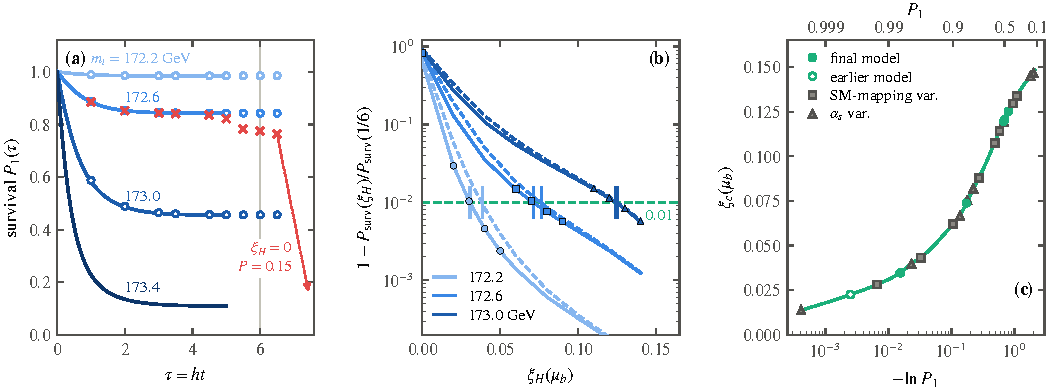
\includegraphics[width=\textwidth]{prd_hazard_realtime}
\caption{Survival along the turning solution and the role of $\xiH$.
(a)~Hazard survival $\Pone(\tau)$ for $m_t=172.2$--$173.4\GeV$ with the norm of the real-time evolution at $\xiH=1/6$ (circles) and $\xiH=0$ (crosses; arrow: final value after the classical stage, which starts at $\tau=6$). %
(b)~Relative loss $1-P_{\rm surv}(\xiH)/P_{\rm surv}(1/6)$ from one-dimensional (lines; solid and dashed: two prescriptions for $\lambda$) and two-dimensional (markers) real-time evolution; the $1\%$ line defines $\xic$ (ticks).
(c)~$\xic$ depends on $m_t$, $\alpha_s$, and the Standard Model mapping only through $\Pone$, tested for $0.45\lesssim\Pone\lesssim0.998$ (final model; earlier model and its variants).} %
\label{fig:rb-hazard}
\end{figure}

\subsection{Two branches}
\label{sec:rb-branches}

A turning point is time symmetric, and in the reading of assumption (A4) both halves $\tau<0$ and $\tau>0$ are expanding branches (Sec.~\ref{rep:gate}).
By time-reflection symmetry $\Pone$ is the same for both.
We show that their joint survival is not a probability in the decoherent-histories sense~\cite{Gell-Mann:1991kdm,Goldstein:1994cp}.

\paragraph{Setup.}
With $\xiH=1/6$ the zero-mode Hamiltonian $H(\eta)$ is real and even in $\eta$.
With complex conjugation $K$ the propagator obeys $KU(\eta_2,\eta_1)K=U(-\eta_2,-\eta_1)$, since both sides solve the same equation with the same initial value.
Let $P$ project onto $r<r_{\rm top}$ and define the Heisenberg projectors at the turning point
\begin{equation}
E_+=U(T,0)^\dagger PU(T,0),\qquad E_-=KE_+K .
\label{eq:rb-Epm}
\end{equation}
For a real $\psi_0$ the single-branch probabilities are equal, $\Pone=\langle\psi_0|E_+|\psi_0\rangle=\langle\psi_0|E_-|\psi_0\rangle$.
A probability for the joint event needs a decoherent set of histories~\cite{Gell-Mann:1991kdm}.
The two-time set $C_{ab}=P_b(T)P_a(-T)$, with $a,b\in\{{\rm in},{\rm out}\}$, has decoherence functional $D(h,h')=\langle C_{h'}\psi_0|C_h\psi_0\rangle$.
With $A=P\psi(T)$, time reflection gives $P\psi(-T)=A^*$.
Define $X=PU(T,-T)A^*$ and $Y=A-X$.
Then
\begin{equation}
D({\rm in},{\rm in})=\|X\|^2,\qquad D({\rm out},{\rm in})=\|Y\|^2,\qquad
D_{\rm off}=\langle Y|X\rangle=\langle A|X\rangle-\|X\|^2,
\label{eq:rb-decoh}
\end{equation}
and the linear value is $K_{\rm lin}=\langle E_+\psi_0|E_-\psi_0\rangle=\langle A|X\rangle$.
Only two forward evolutions from states localized in the well are needed, and the absorber is exact for them because outgoing flux never returns.
The interference ratio is $\varepsilon=|D_{\rm off}|/[D({\rm in},{\rm in})D({\rm out},{\rm in})]^{1/2}$.

\paragraph{Three statements.}
(i)~For a real $\psi_0$ the reversed set $P_a(-T)P_b(T)$ has the complex-conjugate functional with the branch labels exchanged, so the order of times plays no role.
(ii)~If the in-well part is the adiabatic resonance after the initial transient, $P\psi(T)=c\,P_h(T)^{1/2}e^{-i\theta}\varphi_T$ with $|c|^2=w_0$, and the resonance decays from $-T$ to $T$ with $P_h(T)^2$, then $X\parallel A$ and $\varepsilon=1$: the set has maximal interference.
In this limit $D({\rm in},{\rm in})=\Pone^3/w_0^2$ and ${\rm Re}\,K_{\rm lin}=(\Pone^2/w_0)\cos2\alpha$ with $\alpha=\arg c$.
For $w_0=1$ the diagonal element $\Pone^3$ falls below the Fr\'echet bound $2\Pone-1$ when $\Pone>(\sqrt5-1)/2=0.618$, so it cannot be a probability. %
Physically, the decayed component of the $-$ branch at $-T$ is, read forward, the incoming flux that refills the resonance at the turning point; both outcomes of the $-$ branch feed the same surviving state of the $+$ branch, which keeps no record of them.
(iii)~A joint distribution with marginals $E_-$ and $E_+$ for all states exists only if $[E_+,E_-]=0$: from $0\le M_{a,{\rm in}}\le E_+$ it follows that $M_{a,{\rm in}}=E_+M_{a,{\rm in}}E_+$, and similarly for out, so that $E_-^a$ commutes with $E_+$.
In the resonance limit $\|[E_+,E_-]\psi_0\|^2\simeq2\Pone^3(1-\Pone)$, which is $0.19$ at $\Pone=0.84$. %
Quantum mechanics then fixes only the Fr\'echet bounds
\begin{equation}
\max(0,2\Pone-1)\le P_2\le\Pone
\label{eq:rb-frechet}
\end{equation}
on any joint probability $P_2$ with marginals $\Pone$.
Among bilinear assignments $\frac12\{E_+,E_-\}+c\,i[E_+,E_-]$ that reduce to the joint spectral measure for commuting projectors, symmetry under exchange of the branches fixes $c=0$, which leaves the linear (Margenau--Hill) value $P_2^{\rm lin}={\rm Re}\langle\psi_0|E_+E_-|\psi_0\rangle$ of Ref.~\cite{Goldstein:1994cp}.

\paragraph{Numerics.}
For three top masses, six real initial states, and four numerical variants in the one-dimensional model, $\varepsilon=0.9948$--$0.99997$ for $\tau_T\ge1$, the ratio $D({\rm in},{\rm in})\,w_0^2/\Pone^3$ is $1$ to $10^{-4}$, ${\rm Re}\,K_{\rm lin}\,w_0/\Pone^2=0.99993$--$1.000002$, and $|{\rm Im}\,K_{\rm lin}/{\rm Re}\,K_{\rm lin}|\le0.012$. %
A propagation by dense eigendecomposition of the frozen $\tau=0$ Hamiltonian, independent of the Crank--Nicolson stepping, gives $\varepsilon=0.99983$--$0.999996$ and the same linear value to $2\times10^{-5}$. %
The four linear cells are non-negative and lie inside the Fr\'echet band of Eq.~(\ref{eq:rb-frechet}).
If the linear value $P_2=\Pone^2/w_0$ is adopted with $w_0=1$, $m_c(P_2=p)=m_c(\Pone=\sqrt p)$; in the final model this gives $172.380$, $172.764$, and $173.131\GeV$ for $P_2=0.9$, $0.5$, and $0.1$, which is $0.122$, $0.195$, and $0.288\GeV$ below the single-branch values. %
The Fr\'echet band alone allows shifts between $-0.126$ and $0\GeV$ for $P_2=0.9$ and between $-0.241$ and $0\GeV$ for $P_2=0.5$. %
These statements, derived in the one-dimensional zero-mode model, carry over to the two-dimensional model, which has the same time-reflection symmetry and a single resonance.

The shape sector differs in this respect: there the branch that does not cross the turn never failed in any run, so the two-branch survival of the shape equals the single-branch survival of the crossing branch to $4\times10^{-4}$ (Sec.~\ref{rep:quantum-shape}), whereas for the Higgs zero mode both branches decay and their joint survival has no probability. %
We quote single-branch probabilities throughout.
